\apendice{Especificación de diseño}

\section{Introducción}

Este anexo explica como se han resuelto los requisitos y objetivos del proyecto, describiendo detalladamente los datos manejados por el sistema, la arquitectura y su diseño procedimental.

\section{Diseño de datos}

Los datos que se manejan tanto en el servidor como en la aplicación son prácticamente los mismos.
Esto es debido a que para la comunicación entre aplicación y servidor, debe de establecerse un tipo de antes igual para enviar y recibir, ya que estamos ante una comunicación Java-Python. 
Dicha comunicación exige que todos los datos sean serializados, en este caso codificados en bytes, antes del envío.\\

Para la comunicación entre servidor y aplicación, a la hora de solicitar acciones o imágenes, se han utilizado \textit{Strings}, por su facilidad a la hora de ser leídos a través de un \textit{buffer} e incluso a la hora de ser tratados, respecto a otros tipos de datos.
Esta decisión se ha tomado también debido a que determinados tipos de datos no pueden ser enviados por sockets o almacenados en bases de datos (por ejemplo, SQLite no permite tipo datos booleano).\\

Para el envío de imágenes, se ha utilizado la función \textit{imencode} de la librería \textit{OpenCV}, que directamente convierte el frame y lo almacena en un buffer que se le pasa como parámetro a la función.\\

Para las bases de datos de la aplicación y el servidor se han utilizado cadenas de caracteres (\textit{Strings}) y números (\textit{Integers}). A continuación vamos a ver que el conjunto de entidades que se manejan tanto en la aplicación como en el servidor:

\subsection{Entidades en el servidor}

En el servidor se maneja la entidad \textit{Camera} (\ref{fig:bbdd1} y \ref{basedatoscamarasservidor}):
\begin{figure}[!h]
	\centering
	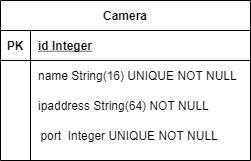
\includegraphics[width=0.5\linewidth]{img/bbdd1}
	\caption{Entidad \textit{Camera} de la base de datos del servidor.}
	\label{fig:bbdd1}
\end{figure}
\tablaSmall{Ejemplo de la base de datos de \textit{cámaras} en el servidor.}{l c c c c}{basedatoscamarasservidor}
{ \multicolumn{1}{l}{Id} & Ip Address & Name & Port \\}{
	0 & 192.168.0.30:8080 & Cámara 1 & 9999\\
	1 & 192.168.0.31:8080 & Cámara 2 & 9998\\
	2 & 192.168.0.32:8080 & Cámara 3 & 9997\\
}
Dicha entidad es manejada a través de la librería \textit{SQLAlchemy} gracias a su ORM incorporado, todo ello implementado a través de los archivos \textit{schema.py} y \textit{cameras.py} en la carpeta \textit{Server}.

\subsection{Entidades en la aplicación}

En la aplicación se manejan las entidades \textit{Cameras} (\ref{fig:bbdd2} y \ref{basedatoscamarasapp}) y \textit{ServerInf} (\ref{fig:bbdd3} y \ref{basedatosipserverapp}):
\begin{figure}[!h]
	\centering
	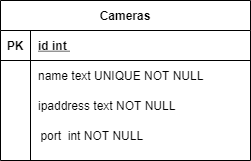
\includegraphics[width=0.5\linewidth]{img/bbdd2}
	\caption{Entidad \textit{Cameras} de la base de datos de la aplicación.}
	\label{fig:bbdd2}
\end{figure}
\begin{figure}[!h]
	\centering
	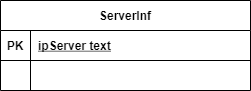
\includegraphics[width=0.5\linewidth]{img/bbdd3}
	\caption{Entidad \textit{ServerInf} de la base de datos de la aplicación.}
	\label{fig:bbdd3}
\end{figure}

\tablaSmall{Ejemplo de la base de datos de \textit{cámaras} en la app.}{l c c c c}{basedatoscamarasapp}
{ \multicolumn{1}{l}{Id} & Ip Address & Name & Port \\}{
	0 & 192.168.0.30:8080 & Cámara 1 & 9999\\
	1 & 192.168.0.31:8080 & Cámara 2 & 9998\\
	2 & 192.168.0.32:8080 & Cámara 3 & 9997\\
}

\tablaSmall{Ejemplo de la base de datos de \textit{dirección ip} del servidor en la app.}{l c c c c}{basedatosipserverapp}
{ \multicolumn{1}{l}{Ip Server}\\}{
	192.168.0.30\\
}

Dichas entidades se manejan a través de la librería \textit{SQLite} gracias a los archivos \textit{DataBaseCameras.java} y \textit{DataBaseCameraInterface.java} en la carpeta \textit{/AndroidApp/app/src/main/java/com/example/appstream/} que implementan la lógica de acceso a la base de datos.\\

Además en la aplicación se mantiene un \textit{ListView} con instancias de la entidad \textit{Camera} que es un clase java para la implementación del botón \ref{fig:botoncamera} de acceso a la imagen de las cámaras, dicha clase se implementa en el archivo \textit{Camera.java} en la carpeta \textit{/AndroidApp/app/src/main/java/com/example/appstream/}.

\begin{figure}[!h]
	\centering
	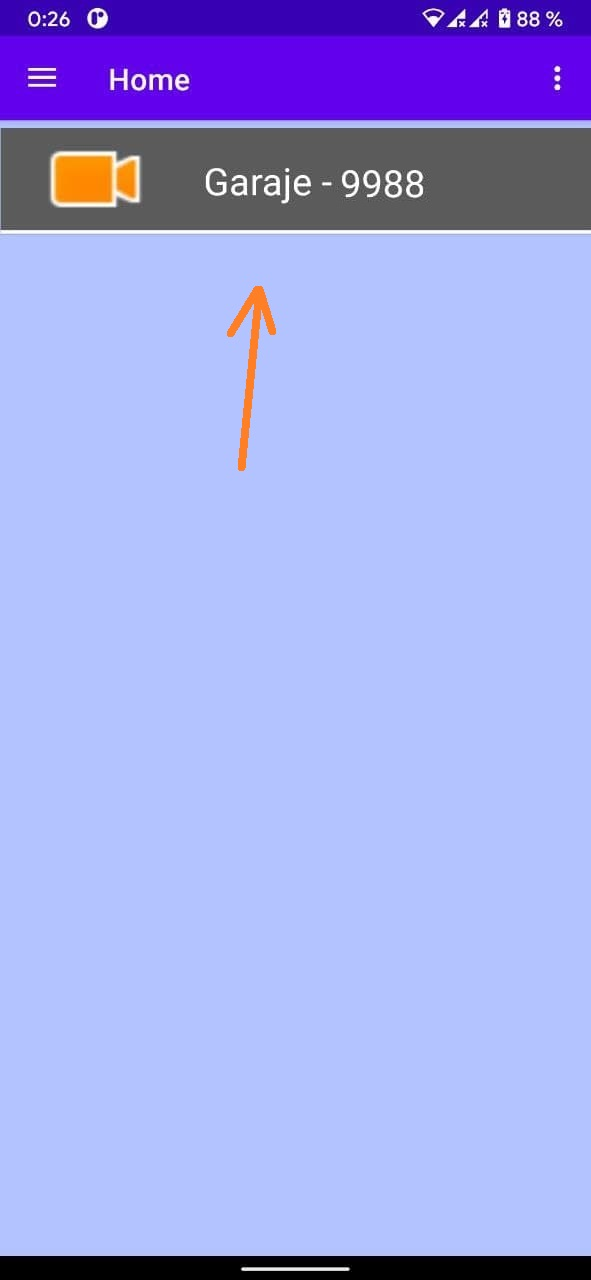
\includegraphics[width=0.35\linewidth]{img/tipodatCamJava}
	\caption{Botón de acceso a la imagen de las cámaras.}
	\label{fig:botoncamera}
\end{figure}



\section{Diseño procedimental}

El diseño procedimental del sistema nos permite apreciar el funcionamiento interno del sistema.\\

A continuación se van a exponer los diagramas de secuencia en los que se representa la interacción entre los distintos elementos del sistema, teniendo en cuenta los requisitos del sistema.\\

\begin{landscape}
\imagengrande{1.8}{diagramaRF11}{Diagramas de secuencia relativo al RF-1.1 (\ref{RF1-1}).}
\imagengrande{1.8}{diagramaRF12}{Diagramas de secuencia relativo al RF-1.2 (\ref{RF1-2}).}
\imagengrande{1.8}{diagramaRF21}{Diagramas de secuencia relativo al RF-2.1 (\ref{RF2-1}).}
\imagengrande{1.2}{diagramaRF22}{Diagramas de secuencia relativo al RF-2.2 (\ref{RF2-2}).}
\imagengrande{1.8}{diagramaRF30}{Diagramas de secuencia relativo al RF-3.1 (\ref{RF3-1}).}
\imagengrande{1.2}{diagramaRF4}{Diagramas de secuencia relativo al RF-4.2 (\ref{RF4-2}).}
\end{landscape}



\section{Diseño arquitectónico}

Esta sección trata el concepto de arquitectura software, usado con el fin de construirlo con la máxima calidad posible cumpliendo los plazos de tiempo establecidos.

\subsection{Arquitectura Cliente-Servidor}

La arquitectura Cliente-Servidor (\ref{fig:arqCliente-servidor}) es un modelo de diseño de software en el que se dividen las  tareas entre dos partes, el proveedor de recursos (o servidor), y los clientes. El cliente solicita los recursos al servidor, y el servidor se encarga de responder la demanda del cliente. El servidores suelen ser máquinas que actúan como sistemas gestores de bases de datos o aplicaciones.
\imagen{arqCliente-servidor}{Imagen explicativa de la arquitectura Cliente-Servidor.}\label{fig:arqCliente-servidor}

El proyecto se ha dividido en la aplicación como cliente y el servidor.

\subsection{Arquitectura Servidor}

Dentro del servidor se ha seguido el patrón de arquitectura modelo-vista-controlador (MVC).

\subsubsection{Patrón modelo-vista-controlador (MVC)}

El patrón MVC \ref{fig:m-v-c} es un patrón arquitectónico que separa el sistema en tres partes, los datos, la lógica de la aplicación y la interfaz de usuario. El modelo es la capa de datos, la vista es la interfaz de usuario y el controlador, la lógica de la aplicación.
\imagen{m-v-c}{Imagen explicativa del patrón MVC.}
En este proyecto se ha utilizado de la siguiente manera:
\begin{itemize}
\item
	Una primera carpeta de datos (\textit{data}) que contiene la base de datos y el ORM (\textit{schema.py}) para el acceso a la misma, todo ello se encuentra dentro de la carpeta \textit{db}.
\item
	Una carpeta llamada \textit{logic} que contiene la lógica de negocio de la aplicación. 
	Dentro de ella encontramos el archivo \textit{MainServer.py}. 
\item
	Una última carpeta que implementa la capa de presentación (\textit{presentation}).
	Dentro de ella encontramos el archivo \textit{CamConnex.py}, que implementa el envío de imágenes a los clientes.
\end{itemize}

\subsection{Arquitectura de la aplicación}

En cuanto a la arquitectura del servidor, no se ha seguido un patrón claro.
Los archivos de la aplicación están en la carpeta \textit{/AndroidApp/app/src/main/java/com/example/appstream/}.

\subsection{Estructura global}

Por último vamos a ver los respectivos diagramas que componen el presente trabajo.

\imagengrande{1}{diagramaClasesServer}{Diagramas de clases del servidor.}

\begin{landscape}
\imagengrande{1.8}{diagramaClasesApp}{Diagramas de clases de la aplicación.}
\end{landscape}